\documentclass{statphysicsdep}



%%%%%%%%%%%%%%%%%%%%%%%%%%%%%%%%%%%%%%%%%%%%%%%%%%%%%%%%%%%%%
% Настройки титулки
\usepackage{review-titlepage}
\TitleWorkTitle{
Сравнительный анализ методов оценки угла прихода излучения на 
антенную решетку пользователя в системах связи стандарта 5G NR 
}

\setauthor{1}{}{Понур К.А.}
%%%%%%%%%%%%%%%%%%%%%%%%%%%%%%%%%%%%%%%%%%%%%%%%%%%%%%%%%%%%%


\usepackage{booktabs} % For \toprule, \midrule and \bottomrule
\usepackage{siunitx} % Formats the units and values
\usepackage{pgfplotstable} % Generates table from .csv
\pgfplotsset{compat=1.18}
\usepackage{tabularx}
% Setup siunitx:
\sisetup{
  round-mode          = places, % Rounds numbers
  round-precision     = 2, % to 2 places
}






% Прочее
\newcommand\mean[1]{\langle #1 \rangle}
\newcommand\const{\text{const}}
\renewcommand{\phi}{\varphi}
\renewcommand{\epsilon}{\varepsilon}
\renewcommand\vec[1]{\vectorbold{#1}}
\setcounter{MaxMatrixCols}{20}

% Настройка переносов некоторых слов
\hyphenation{
  при-ем-ни-ков,
  э-лек-трон-но,
  вы-чис-лит-ель-ной,
  hSearch-MMSE
}

\addbibresource{library.bib}
\usepackage{enumitem}
\usepackage{subcaption}
\usepackage{soulutf8}



% \titlecontents{chapter}[0pt\addvspace{15pt}]
% {\llap{\makebox[3em]{\oldstylenums{\thecontentspage\hfill\thecontentslabel}}\hskip1em}
%   \small\scshape\vskip-\baseline{}skip}{}{}{}
% \titlecontents*{section}[20pt]
% {\upshape}{}{}
% {, \oldstylenums{\thecontentspage}}[][\ \textbullet\ ][]

\def\ACS{\textit{ACS}}
\def\baseline{\textit{baseline}}
\def\hSearchMMSE{\textit{hSearchMMSE}}
\def\AuxBeam{\textit{AuxBeam}}

% \newcommand{\ACS{}}{{ACS}~}
% \newcommand{\baseline{}}{{baseline}~}
% \newcommand{\hSearchMMSE{}}{{hSearchMMSE}~}
% \newcommand{\AuxBeam}{{AuxBeam}~}

\makeatletter
\patchcmd{\@setref}{\bfseries ??}{\bfseries\hl{??}}{}{}
\makeatother
\begin{document}



\maketitle
\newpage

\small
{
\hypersetup{linkcolor=black}
\tableofcontents
}
\normalsize

% \nomenclature[A]{LLS}{Link Level Simulator}
\nomenclature[A]{УМ}{Усилитель Мощности}
\nomenclature[A]{КУ}{Коэффициент Усиления}
\nomenclature[A]{АХ}{Амплитудная Характеристка}
\nomenclature[A]{ФХ}{Фазовая Характеристка}
\nomenclature[A]{OBO}{Output Back-Off}
\nomenclature[A]{IBO}{Input Back-Off}
\nomenclature[A]{5G NR}{5G New Radio}
\nomenclature[A]{OFDM}{Orthogonal Frequency Division Multiplexing}
\nomenclature[A]{CP}{Cyclic Prefix}
\nomenclature[A]{PD}{Pre-Distortion}
% \nomenclature[A]{AATLF}{Adaptive Angle Tracking Loop Filter}
% \nomenclature[A]{AIC}{Akaike’s Information Criterion}
% \nomenclature[A]{AIP}{Antenna in Package}
% \nomenclature[A]{AOA}{Angle of Arrival}
% \nomenclature[A]{AOD}{Angle of  Departure}
% \nomenclature[A]{AWGN}{Additive White Gaussian Noise}
% \nomenclature[A]{BRP}{Beam Refinement Protocol}
% \nomenclature[A]{CCATLF}{Constant Coefficient Angle Tracking Loop Filter}
% \nomenclature[A]{CDF}{Cumulative Distribution Function}
% \nomenclature[A]{CFAR}{Constant False Alarm Ratio}
% \nomenclature[A]{CoMP}{Coordinated Multipoint}
% \nomenclature[A]{CSI}{Channel State Information}
% \nomenclature[A]{DCO}{Digitally Controlled Oscillator}
% \nomenclature[A]{DKED}{Double Knife-Edge Diffraction}
% \nomenclature[A]{DVR}{Digital Video Recorder}
% \nomenclature[A]{EG}{Equal Gain}
% \nomenclature[A]{EKF}{Extended Kalman Filter}
% \nomenclature[A]{FFT}{Fast Fourier Transform}
% \nomenclature[A]{GCS}{Global Coordinate System}
% \nomenclature[A]{HBF}{Hybrid Beamforming}
% \nomenclature[A]{HDTV}{High Definition Television}
% \nomenclature[A]{KF}{Kalman Filter}
% \nomenclature[A]{LCS}{Local Coordinate System}
% \nomenclature[A]{LF}{Loop Filter}
% \nomenclature[A]{LOS}{Line-of-Sight}
% \nomenclature[A]{MDL}{Minimum Description Length}
% \nomenclature[A]{ML}{Maximum Likelihood}
% \nomenclature[A]{MMSE}{Minimal Mean Square Error}
% \nomenclature[A]{MPM}{Minimal Polynomial Method}
% \nomenclature[A]{MS}{Maximal Selection}
% \nomenclature[A]{MUSIC}{MUltiple SIgnal Classification}
% \nomenclature[A]{MVDR}{Minimum Variance Distortionless Response}
% \nomenclature[A]{NLOS}{Non Line-of-Sight}
% \nomenclature[A]{NR}{New Radio}
% \nomenclature[A]{PBCH}{Physical Broadcast Channel}
% \nomenclature[A]{PDF}{Probability Density Function}
% \nomenclature[A]{PSS}{Primary Synchronization Signal}
% \nomenclature[A]{RGB-D}{Red-Green-Blue-Depth}
% \nomenclature[A]{RS}{Reference Signal}
% \nomenclature[A]{SLS}{Sector Level Sweep}
% \nomenclature[A]{SSS}{Secondary Synchronization Signal}
% \nomenclature[A]{SVD}{Singular Value Decomposition}
% \nomenclature[A]{TDM}{Time Division Multiplexing}
% \nomenclature[A]{ULA}{Uniform Linear Array}
% \printnomenclature

\Introduction

Massive MIMO — один из многообещающих методов повышения спектральной
эффективности и производительности сети для достижения целевой пропускной
способности в несколько гигабит/с для систем пятого поколения.  В системах 5G
New Radio (NR) есть одно из главных отличий по сравнению с системой предыдущего
поколения (4G) — это использование высокочастотных диапазонов миллиметровых волн
(mmWave) в дополнение к диапазонам ниже 6 ГГц. 

В системах пятого поколения связи 5G New Radio для повышения спектральной
эффективности и производительности  сети чаще всего применяются многоэлементные 
антенные решетки с аналого-цифровым формированием луча.   

Стандарт 5G NR предназначен для адаптации к различным способам
формирования диаграммы направленности. Методы формирования ДН,
используемые в миллиметровом канале, играют чрезвычайно
важную роль из-за особенностей распространения и больших потерь мощности.
Кроме того быстрые изменения канала оказывают сильнейшее влияние на
производительность системы.  Поэтому точность формирования ДН
играет крайне важную роль во всей технологии миллиметровой связи. 

В системах миллиметрового диапазона поиск пары лучей пользователя (UE)
и базовой станции (BS) выполняется с помощью сканирования пар
возможных лучей и выбором оптимальной пары. Зачастую это делается путем полного
перебора \textit{всех} возможных пар.  Такая процедура требует значительного
времени и уязвима для быстро изменяющихся каналов таких как, например,
вращение пользователя или блокировка пользователя препятствием. 


Целью исследования является разработка  быстрого,
точного и эффективного с точки зрения вычислительной сложности алгоритма
формирования диаграммы направленности и оценки угла угловой координаты источника
излучения.  

Кроме того, проводится сравнительный анализ эффективности всех исследуемых и
разработанных алгоритмов в квазиоптической модели канала IEEE 802.11ay <<Hotel
Lobby>>, разработанной специально для систем 5G NR на несущей частоте 28 ГГц.

%! TeX root = ../main.tex
\section{Обзор методов оценки угла прихода}


\subsection{Характеристики канала связи миллиметровых длин волн}
Миллиметровая модель канала имеет ряд особенностей, которые описаны во множестве
литературных источников и мировых стандартах \cite{Maltsev2010, Maltsev2017,
    Xu2002, Akdeniz2014, Rappaport2015}. Основные особенности следующие:
\begin{itemize}
    \item Малое влияние дифракции
    \item Высокие потери в канале связи
    \item Потери на шероховатостях отражающих поверхностей
    \item Пути распространения могут быть ассоциированы с геометрическими лучами
\end{itemize}

Последний пункт является наиболее важным с точки зрения алгоритмов оценки угла прихода волны 
(Angle of Arrival).
Также, из этого свойства канала следует, что количество различимых сильных путей
распространения относительно невелико. Это подтверждено результатами
измерений каналов как для внутренних, так и для наружных сценариев.

Например, результаты измерения AOA в помещении представлены на рис.
\ref{fig:3.1}.  На рис. \ref{fig:3.2} представлены уникальные AOA в случае
уличного сценария <<Манхеттен>>. Можно заметить, что среднее число хорошо
различимых независимых путей распространения $\mu=4.7$, что достаточно
мало.



\begin{figure}[ht!]
    \centering
    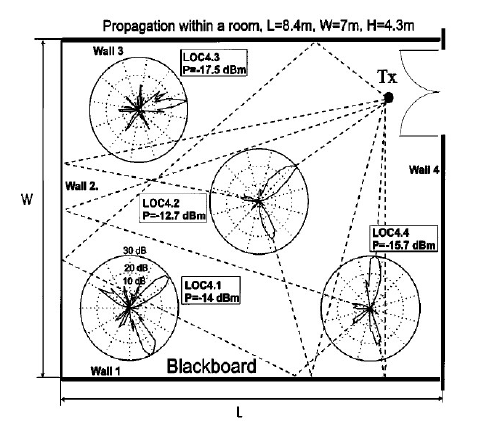
\includegraphics[width=0.6\linewidth]{figs/fig3.1}
    \caption{ Измерение AOA для определения пути распространения в помещении,
        измеренная мощность показана в полярных координатах, $P$ -- максимум
        измеренной мощности. Геометрические лучи показаны только для позиций
        4.2 и 4.4 \cite{Xu2002}.}
    \label{fig:3.1}
\end{figure}

\begin{figure}[ht!]
    \centering
    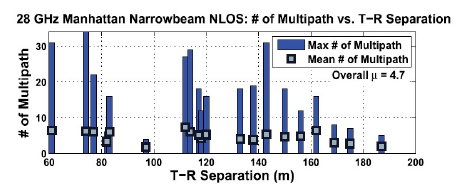
\includegraphics[width=0.8\linewidth]{figs/fig3.2}
    \caption{
        Зависимость числа различимых путей распространения для различных углов азимута и элевации от расстояния между источником и приемником.
        Среднее значение по всем измерениям составило $\mu=4.7$. Измерения проводились с узкой диаграммой направленности в Махеттене \cite{Rappaport2015}.}
    \label{fig:3.2}
\end{figure}

На основе рассмотренных работ, можно сделать вывод, что в данной модели
канала чаще всего можно выделить несколько сильнейших путей
распространения и определить их AOA.

\subsection{Обзор методов оценки угловой координаты источника излучения}
\label{sec:review}

Канал в миллиметровом диапазоне можно представить в виде
набора геометрических лучей.  Самые сильные лучи могут быть
использованы для передачи данных. Как правило, диаграмма направленности
антенны формируется по направлению луча прямой видимости (Line of Sight).
Однако в случае не прямой видимости (Non Line of Sight), может быть
выбран самый сильный отраженный геометрический луч. 

Оценка угла прихода, часто рассматривается в задачах
радиолокации.  Для этих задач  давно разработаны алгоритмы и аппаратные реализации
ещё во времена зарождения радиолокации. Эти алгоритмы совершенствовались с
появлением фазированных антенных решеток.  
Этот может оказаться очень  полезным c учетом  аппаратных ограничений систем
связи 5G NR -- число цифровых портов обычно мало по сравнению с имеющимся
количеством элементов антенной решетки. 

Другой набор алгоритмов пришел из задач спектрального анализа.  В них обычно
предполагается, что сигнал каждой антенны принимается независимо.  Эти алгоритмы
очень эффективны и дают возможность оценить направления на несколько целей
(лучей) одновременно и имеют сверхразрешающую способность, но c другой стороны,
они требуют значительных вычислительных ресурсов.  

В этом разделе мы рассмотрим и систематизируем существующие подходы к оценке
АОА, которые нам удалось найти в открытых литературных источниках.  Будут
представлены их преимущества и недостатки.  На этапе моделирования в следующей
части этой работы, мы сократим этот список и выделим наиболее перспективные
методы.

\subsubsection{Методы Фурье и Бартлетта}
\label{sec:3.2.1} \label{sec:Fourier}

Простейшая алгоритм оценки AOA в зарубежной литературе называется бимформингом \cite{Tuncer2009, Stoica2005} или методом Фурье \cite{Allen2006}.
Основная идея заключается в максимизации мощности, принятой с определенного
направления.

Обозначим сигнал $\vec{y}(t)$ принятой антенной решеткой от некоторого
удаленного источника
\begin{equation}
    \label{eq:3.1}
    \vec{y}(t) = a(t) \vec{s}(\phi_{src}) + \vec{\xi}(t),
\end{equation}
где ${\vec{s}(\phi_{src})}$ -- фазирующий вектор,
$\phi_{src}$ -- угол прихода (AOA); $\vec \xi$ -- вектор шума.
Каждый элемент фазирующего вектора представляется в виде
\begin{equation}
    \label{eq:3.2}
    \qty{\vec{s}(\phi)}_n = \exp{-i(\vec k (\phi), \vec \rho_n)},
\end{equation}
где $\vec k (\phi_{src})$ -- волновой вектор плоской волны, $\vec\rho_n$ радиус-вектор
$n$-го элемента антенны.
В случае эквидистантной антенной решетки, последнее уравнение приведется
к виду
\begin{equation}
    \qty{\vec s(\phi)}_n = \exp{i2\pi\frac{d}{\lambda}\sin(\phi)n},
\end{equation}
где $d$ -- расстояние между элементами антенной решетки, $\lambda$ -- длина
волны излученного сигнала.

Чтобы получить максимальную мощность с некоторого направления $\phi$ необходимо
сформировать соответствующую диаграмму направленности с помощью
весового вектора антенной решетки $\vec w (\phi) = \vec s(\phi)/\rVert(\vec
    s(\phi))\lVert$.  Тогда, можно найти мощность излученного с АР сигнала.
\begin{equation}
    p(\phi) = \abs{\vec w^H (\phi) \vec y}^2.
\end{equation}

Оценкой AOA будет являться значение аргумента $\phi$, обеспечивающего максимум функции $p(\phi)$
\begin{equation}
    \phi^* = \arg\max p(\phi)
\end{equation}

\begin{figure}[ht!]
    \centering
    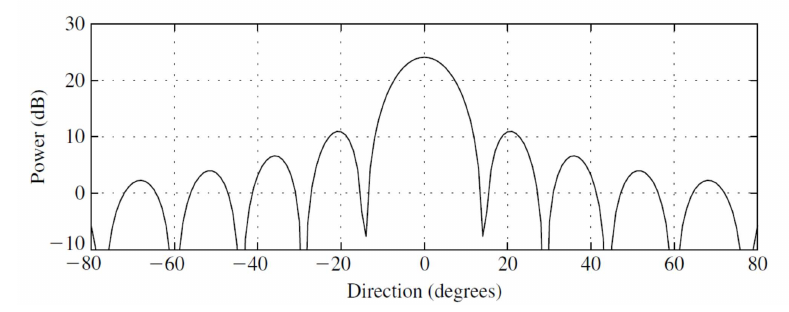
\includegraphics[width=\linewidth]{figs/fig3.9}
    \caption{ДН для 16-ти элементной эквидистантной линейной
        решетки ($\frac{d}{\lambda}=0.5$), сформированной в направлении $0^\circ$
        \cite{Tuncer2009}. }
    \label{fig:3.9}
\end{figure}

Для фазированной антенной решетки поиск $\phi^*$ может быть реализован во временной
области с помощью сканирования диаграммой направленности. Если количество
приемников (цифровых портов) равно количеству антенных элементов, искомая
функция $p(\phi)$ может быть оценена в цифровой области \cite{Stoica2005}.  В
литературе этот подход также называется методом Бартлетта \cite{Godara2004}.

Функция $p(\phi)$ примет вид
\begin{equation}
    p(\phi) = \frac{\vec s^H(\varphi) \hat{\vec M} \vec s (\phi)}{N^2},
\end{equation}
где $\hat{\vec M}$ -- оценка корреляционной матрицы принятого сигнала
\begin{equation}
    \label{eq:3.7}
    \hat{\vec M} = \frac{1}{L} \sum\limits_{t=1}^{L} \vec y(t) y^H (t)
\end{equation}

\paragraph{Преимущества}%
\begin{enumerate}
    \item Теоретически, метод Фурье и метод Бартлетта являются оптимальными
          решениями для оценки AOA в случае однолучевого канала.
    \item Легко технически реализуется на конечном устройстве и требует мало
          вычислительных мощностей.
\end{enumerate}

\paragraph{Недостатки}%

\begin{enumerate}
    \item На практике, точность поиска снижается.
          Это происходит, во-первых,  потому что производная функции $p(\phi)$
          в направлении на максимум равна нулю и из-за <<плоской>> вершины сложно
          точно определить точку экстремума. Во-вторых, необходимо
          обеспечить высокую дискретизацию по углу для обеспечения приемлемой
          оценки.
    \item Алгоритм может не подойти в случае быстро движущихся пользователей, если поиск реализован с помощью сканирования во временной области.
    \item Метод обеспечивает разрешающую способность, зависящую
          от ширина главного лепестка ДН. Увеличение отношения сигнал/шум (ОСШ) или времени
          сканирования не приведет к качественному улучшению разрешения.  Это делает
          этот подход малопригодным для оценки многолучевого АОА.
    \item В случае нескольких близко расположенных АОА присутствует
          значительная систематическая ошибка.
\end{enumerate}


\subsubsection{Метод максимального правдоподобия}%
\label{sub:metod_maksimal_nogo_pravdopodobiia}
\label{sec:MLE-algorithm}
При наличии нескольких путей распространения, оптимальная оценка AOA может быть
получена с помощью максимально правдоподобной оценки (Maximum Likelihood
Estimator) \cite{Tuncer2009}.  

Рассмотрим модель сигнала:
\begin{equation}
    \label{eq:3.8}
    \vec y(t) = \sum\limits_{q=1}^{J} a_q(t)\vec s(\phi_q) + \vec \xi(t),
\end{equation}
где $J$ число путей распространения; $a_q(t)$ -- комплексная амплитуда $q$-то
луча, $\vec s(\phi_q)$ -- фазирующий вектор;  $\phi_q$ -- угол прихода (AOA) $q$-то
луча и $\xi(t)$ -- вектор белого гауссового шума.

Для этой модели канала критерий МП может быть записан как критерий минимума
среднеквадратичной ошибки (Minimum Mean Square Error)
\begin{equation}
    d(\phi_1, \hdots, \phi_J) = \sum\limits_{t}^{} \abs{\vec(t) -
        \sum\limits_{q=1}^{J} a_q(t) \vec s(\phi_q)}^2 \to \min_{\phi_q}.
\end{equation}
Что можно переписать в виде
\begin{equation}
    \label{eq:3.10}
    d(\phi_1, \hdots, \phi_J) = \sum\limits_{t}^{} \vec y^H(t) \vec
    P_\perp(\phi_1, \hdots, \phi_J) \vec y(t) \to \min_{\phi_q},
\end{equation}
\begin{equation}
    \vec P_\perp(\phi_1, \hdots, \phi_J) = \vec E - \vec S(\vec S^H \vec S)^{-1}
    \vec S^H,
\end{equation}
где $\vec P_\perp$ -- проекционная матрица, 
$\vec S = \qty[\vec s(\phi_1) \dots \vec s (\phi_J)]$. 

Минимизация $d(\phi_1, \hdots, \phi_J)$ в общем случае производится численно и
как правило требует больших вычислительных ресурсов для реализации $J$-мерной
минимизации \cite{Tuncer2009}. 


\paragraph{Преимущества}%
\begin{enumerate}
    \item Обеспечивает оптимальное решение в случае нескольких сильных путей распространения 
\end{enumerate}

\paragraph{Недостатки}%
\begin{enumerate}
    \item Требует большого количества цифровых портов 
    \item Требует больших вычислительных затрат
    \item Не позволяет оценить количество доминирующих путей распространения. Если их количество неизвестно, метод становится неоптимальным. 
\end{enumerate}

\subsubsection{Метод моноимпульса}%
\label{sec:monopulse}

Данная разновидность формирования ДН часто называется моноимпульсом и обычно 
используется в радиолокационных системах для задач слежения. 
Этот алгоритм использует разницу между мощностью двух измеренных лучей как метрику для 
оценки AOA \cite{Tuncer2009}. Вводится следующая функция 
\begin{equation}
    \label{eq:3.11}
    b(\phi) = \frac{1}{\Delta} \qty(\abs{\vec w^H(\phi+0.5 \Delta)\vec y}^2)
    -
    \qty(\abs{\vec w^H(\phi-0.5 \Delta)\vec y}^2) \approx \dv{p(\phi)}{\phi} ,
\end{equation}
где $p(\phi)$ и $\vec w(\phi)$ были определены в разделе \ref{sec:3.2.1}, $\Delta$ -- некоторый скаляр. Тогда, оценка AOA
заключается в поиске такого угла $\phi$, который обеспечивает нуль функции $b(\phi)$
\begin{equation}
    \label{eq:3.12}
    \phi = \arg\qty{b(\phi) = 0}.
\end{equation}

Величина $\Delta$ может быть порядка ширины луча, но  $b(\phi)$ всё равно будет
хорошо аппроксимироваться производной $p(\phi)$, поскольку $b(\phi)$ почти
линейна в большом диапазоне углов около нуля \cite{Tuncer2009}.  

\begin{figure}[ht]
    \centering
    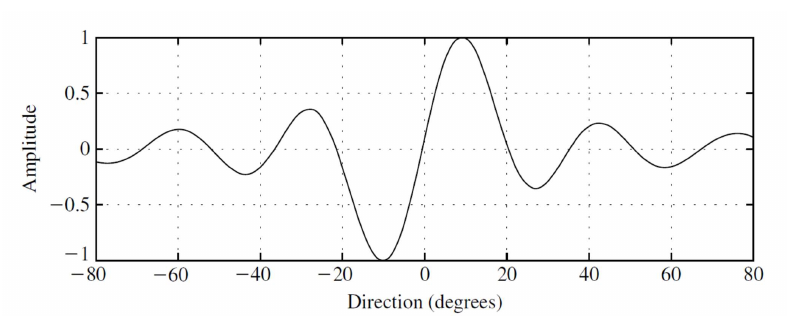
\includegraphics[width=\linewidth]{figs/fig3.11}
    \caption{Зависимость метрики $b(\phi)$ для 16-ти элементной ULA \cite{Tuncer2009}. Направление на источник -- 0 град.}
    \label{fig:3.11}
\end{figure}
% Another variant of the algorithm is often called Monopulse Ratio or Amplitude
% Comparison Monopulse \cite{Mosca1969}. This algorithm requires coherent reception with two
% channels (RF-chains): sum and difference. The sum channel is formed with beam
% pattern which has a maximum for a certain direction. The difference beam
% pattern has a null for this direction. In \cite{Kim2018} the algorithm which uses TDM for
% sum and difference channels is proposed and investigated. It employs cycle
% prefix of OFDM signal to receive two identical signals with different beam
% patterns using a single RF-chain and phased antenna array. This approach seems
% promising, but there are some issues related to phase shifter switching delay
% and multipath propagation influence.
% The metric of monopulse ratio is \cite{Kim2018}
% \begin{equation}
%     \label{eq:}
%     \tan(\frac{N}{4}(\phi_{src} - \phi)) =
%     \frac{Im\qty{\sum\limits_{k} y_d(k) y_s^*(k)}}{\sum\limits_{k}
%         \abs{y_s(k)}^2},
% \end{equation}
% where $\phi_{src}$ is actual  AOA;  $\phi$ is roughly estimated AOA via beam
% sweeping (it is the direction of the sum beam); N is number of antenna
% elements; $y_s(k)$ and  $y_d(k)$ are signals f the sum and difference channels
% respectively.
% \begin{equation}
%     \label{eq:}
%     y_s(t) = a(t) \vec w_s^H \vec s(\phi_{src}) + \vec w_s^H \vec \xi(t)
% \end{equation}
% \begin{equation}
%     \label{eq:}
%     y_d(t) = a(t) \vec w_d^H \vec s(\phi_{src}) + \vec w_d^H \vec \xi(t)
% \end{equation}

% For a linear antenna array the corresponding beamforming vectors are
% \begin{equation}
%     \label{eq:}
%     \qty{\vec w_s (\phi)}_n = \exp{i_2\pi \frac{d}{\lambda}} \sin \phi
% \end{equation}
% \begin{equation}
%     \label{eq:}
%     \qty{\vec w_d (\phi)}_{n < \frac n {N}{2}} = - \exp{i_2\pi n \frac{d}{\lambda}} \sin \phi
% \end{equation}
% \begin{equation}
%     \label{eq:}
%     \qty{\vec w_d(\phi)}_{n\geq \frac{N}{2}} = +\exp{i2\pi \frac{d}{\lambda}
%         \sin \phi (n - 0.5N)},
% \end{equation}

% \begin{figure}[htpb]
%     \centering
%     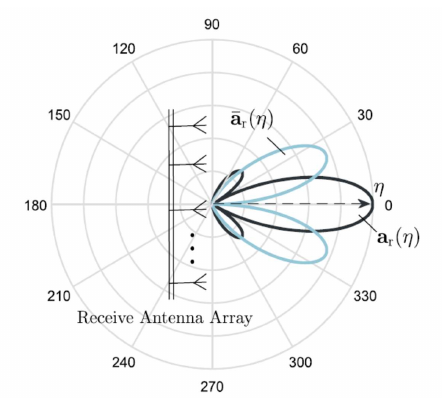
\includegraphics[width=0.6\linewidth]{figs/fig3.12}
%     \caption{Sum and difference beam patterns for monopulse ratio algorithm
%         \cite{Zhu2016}}
%     \label{fig:}
% \end{figure}

% Monopulse ratio is typically used to estimate a single AOA or resolvable angles
% (far spaced targets which are not located within the same beam). However, there
% are some modifications that use a complex monopulse ratio and allow one to
% detect the multiple targets in a certain beam and estimate their angle
% positions \cite{Luoshengbin2016} \cite{Sherman2011}.  


В \cite{Zhu2016} представлена ещё одна реализация метода моноимпульса, не требующая 
поиска нуля функции \eqref{eq:3.11}
\begin{equation}
    \label{eq:3.19}
    \zeta_n = \frac{p(\eta_n - \delta) - p(\eta_n + \delta)}{p(\eta_n - \delta)
        + p(\eta_n + \delta)} =
    \frac{\sin(\psi - \eta_n)\sin\delta}{1 - \cos(\psi - \eta_n)\cos \delta}
\end{equation}

\begin{equation}
    \label{eq:3.20}
    \psi = \eta_n - \arcsin(
    \zeta_n \frac{\sin\delta}{\sin^2 \delta + \zeta^2_n \cos^2\delta}
    -
    \frac{\zeta_n \sqrt{1-\zeta^2_n} \sin \delta \cos \delta}{\sin^2\delta +
        \zeta^2_n \cos^2 \delta}
    )
\end{equation}
где $\psi_n = 2\pi \frac{d}{\lambda} \sin \phi$ -- обобщенный угол 
главного лепестка с азимутальным направлением $\phi$,  $\eta$ -- центральный угол между двумя лучами моноимпульса, 
$n$ -- индекс лучшей пары лучей, $\delta = \frac{\pi}{N}$, $N$ -- число элементов в АР, $p(\eta)$ 
мощность сигнала, измеренной с луча, направленного на обобщенный угол $\eta$.

\begin{figure}[ht!]
    \centering
    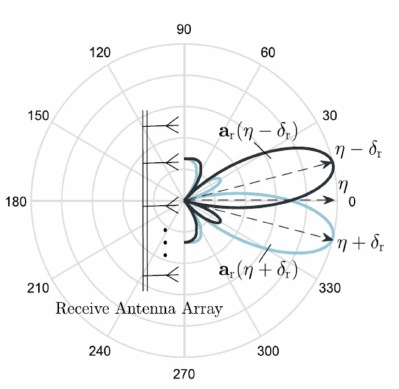
\includegraphics[width=0.45\linewidth]{figs/fig3.13}
    \caption{Сформированные лучи моноимпульса \cite{Zhu2016}}
    \label{fig:}
\end{figure}

Как показано в  \cite{Sherman2011},
этот метод может давать неправильный результат, если фактический AOA
находится вблизи максимума одной из двух сформированных ДН, а ОСШ достаточно низкое. 
В \cite{Sherman2011} для решения этой проблемы предлагается использовать ещё два дополнительных луча (см. рис. \ref{fig:3.14}).

\begin{figure}[ht!]
    \centering
    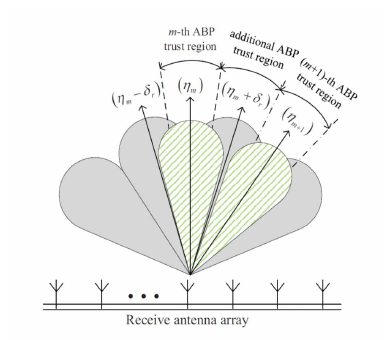
\includegraphics[width=0.6\linewidth]{figs/fig3.14}
    \caption{Метод монопульса с дополнительной парой лучей \cite{Tuncer2009}}
    \label{fig:3.14}
\end{figure}

\paragraph{Преимущества}%
\label{par:preimushchestva}

\begin{enumerate}
    \item На практике, этот метод более точный, чем методы Барлетта или Фурье, поскольку производная достаточно быстро изменяется вблизи AOA.
    \item Может быть реализован на фазированной антенной решетке с одним цифровым портом.
    \item Для оценки необходимо небольшое количество измерений. 
\end{enumerate}

\paragraph{Недостатки}%
\label{par:nedostatki}
\begin{enumerate}
    \item Поскольку является вариацией метода Фурье, его точность будет зависеть 
    от ширины главного лепестка ДН. Увеличение ОСШ или времени оценки не приведет к улучшению результата. 
    \item В случае двух близко расположенных источников сигнала, может наблюдаться значительная систематическая ошибка. 
\end{enumerate}

\subsubsection{Метод Кейпона}%
\label{sub:minimum_variance_distortionless_response_estimator_capon_method_}
\label{sec:Capon}

Другой алгоритм, основанный на методе Фурье -- Minimum Variance
Distortionless Response Estimator (MVDR), также называемый методом Кейпона \cite{Stoica2005,Allen2006, Godara2004}. 
Основная идея заключается в том, чтобы с помощью формирования ДН 
минимизировать мощность со всех направлений, при постоянном усилении для некоторого направления $\phi$.

\begin{figure}[h]
    \centering
    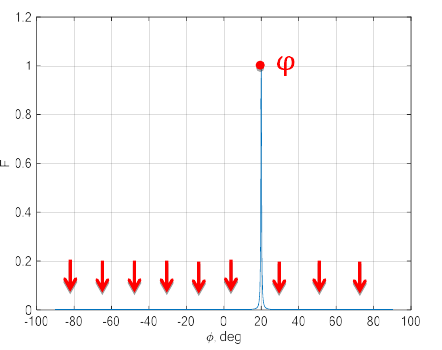
\includegraphics[width=0.6\linewidth]{figs/fig3.15.png}
    \caption{Основная идея метода Кейпона}
    \label{fig:3.15}
\end{figure}
Выбор весовой вектора в этом случае становится задачей нелинейного программирования 
\cite{Stoica2005, Godara2004}
\begin{equation}
    \label{eq:3.21}
    \vec w(\phi) = \frac{\hat{\vec M}^{-1} \vec s (\phi)}{\vec s^H(\phi)
        \hat{\vec M}^{-1} \vec s(\phi)},
\end{equation}
где $s(\phi)$ -- фазирующий вектор, определенный в \eqref{eq:3.2}, $\vec{\hat M}$ корреляционная матрица \eqref{eq:3.7}.
Искомая функция принимает следующий вид
\begin{equation}
    \label{eq:3.22}
    p(\phi) = \frac{1}{s^H(\phi) \vec M^{-1} \vec s(\phi)}
\end{equation}
Выражение \eqref{eq:3.22} представляет собой принятую мощность. Пики этой функции соответствуют найденными углам прихода. 
\paragraph{Преимущества}%
\begin{enumerate}
    \item Метод Кейпона обеспечивает высокую точность оценки AOA.
    \item Может быть использован для нахождения нескольких AOA, благодаря сверхразрешению. 
    \item Может быть реализован аппаратно, поскольку функция \eqref{eq:3.22} имеет смысл принятой мощности.
\end{enumerate}
\paragraph{Недостатки}%
\begin{enumerate}
    \item Разрешение ограничено, даже если корреляционная матрица $\vec M$
    известна точно. Для улучшения разрешения необходимо увеличивать ОСШ или
    количество элементов АР
    \item Нахождение обратной матрицы, которое необходимо для этого метода, требует больших вычислительных затрат.
\end{enumerate}
\section{Проблемы исследования и ожидаемые результаты}

В работе требуется рассмотреть несколько важных сценариев поведения пользователя, 
позволяющих получить полную информацию о качестве работы различных алгоритмов.
Чтобы провести полное статистического исследования различных подходов, требуется
выполнится Монте-Карло моделирование с большим числом независимых
экспериментов.  

Для этих задач необходимо реализовать квазиоптическую модель канала 
IEEE 802.11ay <<Hotel Lobby>>, что является нетривиальной задачей в области 
программирования и статистической радиофизики. 

Ожидается, что оптимальным алгоритмом для определения угла прихода излучения будет 
являться алгоритм моноимпульса, идея которого изложена в \ref{sec:monopulse}.

\Conclusion


В системах пятого поколения связи 5G New Radio
для повышения спектральной
эффективности и производительности  сети чаще всего
применяются многоэлементные
антенные решетки с аналого-цифровым формированием
диаграммы направленности.

Для точного формирования диаграммы направленности, пользователю и базовой
станции необходимо знать направление в котором принятая пользователем мощность
сигнала оказывается максимально возможной.  Помимо этого, в процессе
установления связи нередко возникают ситуации, когда направления с максимальной
мощностью в канале оказываются неактуальными в результате блокировки сигналов
различными препятствиями. В этих случаях, для поддержания стабильного
соединения, помимо наилучшего направления, необходимо оценивать одно или
несколько резервных направлений.

Поэтому оценка угла прихода излучения на антенную решетку является важной
прикладной задачей, позволяющая улучшить качество и скорость связи.



{\footnotesize
\printbibliography
}


\end{document}



% [1]M. Giordani, M. Polese, A. Roy, D. Castor and M. Zorzi, "A Tutorial on Beam Management for
% 3GPP NR at mmWave Frequencies," IEEE Communications Surveys & Tutorials, vol. 21, no. 1,
% pp. 173-196, 2019.
% [2]IEEE doc. 802.11-09/0334r8 Channel Models for 60 GHz WLAN Systems, A. Maltsev et al., May
% 2010.
% [3] IEEE doc. 802.11-15/1150r9 Channel Models for IEEE 802.11ay, A. Maltsev et al., March 2017.
% [4]H. Xu, V. Kukshya and T. S. Rappaport, “Spatial and temporal characteristics of 60-GHz indoor
% channels,” IEEE Journal on Selected Areas in Communications, vol. 20, no. 3, pp. 620 - 630,
% 2002.
% [5]M. R. Akdeniz, Y. Liu, M. K. Samimi, S. Sun, S. Rangan and E. Erkip, “Millimeter Wave
% Channel Modeling and Cellular Capacity Evaluation,” IEEE Journal on Selected Areas in
% Communications, vol. 32, no. 6, pp. 1164 - 1179, 2014.
% [6]T. S. Rappaport, G. R. MacCartney, M. K. Samimi and S. Sun, "Wideband Millimeter-Wave
% Propagation Measurements and Channel Models for Future Wireless Communication System
% Design," IEEE Transactions on Communications, vol. 63, no. 9, pp. 3029 - 3056, 2015.
% [7]Y. M. Tsang and A. S. Y. Poon, “Detecting Human Blockage and Device Movement in
% mmWave Communication System,” in 2011 IEEE Global Telecommunications Conference -
% GLOBECOM 2011, Houston, TX, USA, 2011.
% [8]IEEE doc. 802.11-09/0995r1, 60 GHz Transmission and Reflection Measurements, Tian-Wei
% Huang et al, September 23, 2009.
% [9]M. Jacob, C. Mbianke and T. Kürner, "A dynamic 60 GHz radio channel model for system level
% simulations with MAC protocols for IEEE 802.11ad," in IEEE International Symposium on
% Consumer Electronics (ISCE 2010), Braunschweig, Germany, 2010.
% [10] M. Peter, M. Wisotzki, M. Raceala-Motoc, W. Keusgen, R. Felbecker, M. Jacob, S. Priebe and
% T. Kürner, “Analyzing human body shadowing at 60 GHz: Systematic wideband MIMO
% measurements and modeling approaches,” in 2012 6th European Conference on Antennas and
% Propagation (EUCAP), Prague, Czech Republic, 2012.
% [11] V. Raghavan, L. Akhoondzadeh-Asl, V. Podshivalov, J. Hulten, M. A. Tassoudji, O. H. Koymen,
% A. Sampath and J. Li, "Statistical Blockage Modeling and Robustness of Beamforming in
% Millimeter-Wave Systems," IEEE Transactions on Microwave Theory and Techniques, vol. 67,
% no. 7, pp. 3010-3024, 2019.
% 198
% [12] G. R. MacCartney, S. J, S. Sun and T. S. Rappaport, “Millimeter-wave human blockage at 73
% GHz with a simple double knife-edge diffraction model and extension for directional antennas,”
% in Proc. IEEE Veh. Tech. Conf. (Fall), Montreal, Canada, 2016.
% [13] 3GPP TR 38.901 V16.1.0 Study on channel model for frequencies from 0.5 to 100 GHz, 2019.
% [14] B. Gao, Z. Xiao, C. Zhang, L. Su, D. Jin and L. Zeng, “Double-link beam tracking against
% human blockage and device mobility for 60-GHz WLAN,” in 2014 IEEE Wireless
% Communications and Networking Conference (WCNC), Istanbul, 2014.
% [15] S. Collonge, G. Zaharia and G. E. Zein, “Influence of the Human Activity on Wide-Band
% Characteristics of the 60 GHz Indoor Radio Channel,” IEEE Trans Wireless Comm., vol. 3, no.
% 6, pp. 2396 - 2406, 2004.
% [16] E. Tuncer and B. Friedlander, Classical and modern direction-of-arrival estimation, Burlington,
% USA: Academic Press is an imprint of Elsevier, 2009.
% [17] P. Stoica and R. Moses, Spetral analysis of signals, Upper Saddle River, New Jersey: Prentice
% Hall Inc., 2005, p. 427.
% [18] B. Allen and M. Ghavami, Adaptive array systems: fundamentals and applications, John Wiley
% & Sons, 2006.
% [19] L. C. Godara, Smart Antennas, CRC Press, 2004.
% [20] A. K. R. Chavva, S. K, C. Lim, Y. Lee, J. Kim and Y. Rashid, “Sensor Intelligence Based Beam
% Tracking for 5G mmWave Systems: A Practical Approach,” in Proc. 2019 IEEE Global
% Communications Conference (GLOBECOM), Waikoloa, HI, USA, 2019.
% [21] E. Mosca, “Angle Estimation in Amplitude Comparison Monopulse Systems,” IEEE
% Transactions on Aerospace and Electronic Systems, Vols. AES-5, no. 2, pp. 205-212, 1969.
% [22] H. Kim, J. Kim, K. H. Lee and K. S. Kim, "DOA estimation in Cyclic Prefix OFDM Systems in
% LOS mmWave Channel using Monopulse Ratio," in 2018 International Conference on
% Information and Communication Technology Convergence (ICTC), Jeju, South Korea, 17-19
% Oct. 2018.
% [23] D. Zhu, J. Choi and R. W. Heath, "Auxiliary Beam Pair Enabled AoD and AoA Estimation in
% mmWave FD-MIMO Systems," in 2016 IEEE Global Communications Conference
% (GLOBECOM), Washington, DC, USA, 4-8 Dec. 2016.
% [24] W. Luoshengbin, X. Zhenhai, L. Xinhua and D. Chong, "Detection of unresolved targets for
% plane array radar based on monopulse ratio," in 2016 CIE International Conference on Radar
% (RADAR), Guangzhou, China, 10-13 Oct. 2016.
% 199
% [25] S. M. Sherman and D. K. Barton, Monopulse Principles and Techniques, Artech House
% Publishers, 2011.
% [26] S. Kim, H. Han, N. Kim and H. Park, “Robust Beam Tracking Algorithm for mmWave MIMO
% Systems in Mobile Environments,” in 2019 IEEE 90th Vehicular Technology Conference
% (VTC2019-Fall), Honolulu, HI, USA, 2019.
% [27] M. Rubsamen and A. B. Gershman, “Direction-of-Arrival Estimation for Nonuniform Sensor
% Arrays: From Manifold Separation to Fourier Domain MUSIC Methods,” IEEE Transactions on
% Signal Processing, vol. 57, no. 2, pp. 588-599, 2009.
% [28] J. Lee, J. Park and J. Chun, "Weighted Two-Dimensional Root MUSIC for Joint Angle-Doppler
% Estimation With MIMO Radar," IEEE Transactions on Aerospace and Electronic Systems, vol.
% 55, no. 3, pp. 1474-1482, 2019.
% [29] M. D. Zoltowski, G. M. Kautz and S. D. Silverstein, "Development, performance analysis, and
% experimental evaluation of beamspace Root-MUSIC," in [Proceedings] ICASSP 91: 1991
% International Conference on Acoustics, Speech, and Signal Processing, Toronto, Ontario,
% Canada, 1991.
% [30] V. T. Ermolaev, A. G. Flaksman, A. V. Elokhin and V. V. Kuptsov, "Minimal Polynomial
% Method for Estimating Parameters of Signals Received by an Antenna Array," Acoust. Phys.,
% vol. 64, pp. 83-90, 2018.
% [31] V. T. Ermolayev, A. G. Flaksman, A. V. Elokhin and O. A. Shmonin, "Angular Superresolution
% of the Antenna-Array Signals Using the Root Method of Minimum Polynomial of the Correlation
% Matrix," Radiophysics and Quantum Electronics, vol. 61, no. 3, p. 232–241, 2018.
% [32] V. T. Ermolayev, A. G. Flaksman, A. V. Elokhin and O. A. Shmonin, "An Experimental Study
% of the Angular Superresolution of Two Correlated Signals Using the Minimum-Polynomial
% Method," Radiophysics and Quantum Electronics, vol. 61, no. 11, pp. 841-852, 2019.
% [33] R. Roy and T. Kailath , "Esprit - Estimation Of Signal Parameters Via Rotational Invariance
% Techniques," IEEE Trans. Acoustics, Speech and Signal Processing, vol. 37, no. 7, pp. 984-995,
% 1989.
% [34] A. Alkhateeb, O. El Ayach, G. Leus and R. W. Heath, "Channel Estimation and Hybrid
% Precoding for Millimeter Wave Cellular Systems," IEEE Journal of Selected Topics in Signal
% Processing, vol. 8, no. 5, pp. 831-846, 2014.
% [35] S. Shaham, M. Ding, M. Kokshoorn, Z. Lin, S. Dang and R. Abbas, "Fast Channel Estimation
% and Beam Tracking for Millimeter Wave Vehicular Communications," IEEE Access, vol. 7, pp.
% 141104-141118, 2019.
% [36] Q. Duan, T. Kim, H. Huang, K. Liu and G. Wang, "AoD and AoA tracking with directional
% 200
% sounding beam design for millimeter wave MIMO systems," in 2015 IEEE 26th Annual
% International Symposium on Personal, Indoor, and Mobile Radio Communications (PIMRC),
% Hong Kong, 2015, 2015.
% [37] C. Wang and D. Wang, "Synthetic aperture processing for wireless communication signals with
% passive moving array," Multidim Syst Sign Process, vol. 31, p. 1491–1507, 2020.
% [38] A. Maltsev, A. Pudeyev, R. Weiler, M. Peter, W. Keusgen and I. Bolotin, "Virtual Antenna
% Array Methodology for Outdoor Millimeter-Wave Channel Measurements," in 2016 IEEE
% Globecom Workshops (GC Wkshps), Washington, USA, 2016.
% [39] M. Hua, C. Hsu, W. Liao, C. Yao, T. Yeh and H. Liu, "Direction-of-arrival estimator using array
% switching on software defined radio platform," in 2011 IEEE International Symposium on
% Antennas and Propagation (APSURSI), Spokane, WA, 2011.
% [40] C. Jeong, J. Park and H. Yu, "Random access in millimeter-wave beamforming cellular
% networks: issues and approaches," IEEE Commun. Mag., vol. 53, no. 1, p. 180–185, 2015.
% [41] C. N. Barati and et al, "Directional initial access for millimeter wave cellular systems," in Proc.
% 49th Asilomar Conf. Signals Syst. Comput., Pacific Grove, CA, USA, 2015.
% [42] M. Giordani and M. Zorzi, "Improved user tracking in 5G millimeter wave mobile networks via
% refinement operations," in Proc. 16th Annu. Mediterr. Ad Hoc Netw. Workshop (Med-Hoc-Net),
% 2017.
% [43] Y. Tsang, A. Poon and S. Addepalli, "Coding the beams: Improving beamforming training in
% mmwave communication system," in Proc. IEEE Global Telecomm. Conf. (GLOBECOM),
% Houston, TX, USA, 2011.
% [44] A. K. R. Chavva, K. Shubham, C. Lim, Y. Lee, J. Kim and Y. Rashid, "Sensor Intelligence
% Based Beam Tracking for 5G MmWave Systems: A Practical Approach," in Proc. 2019 IEEE
% Global Communications Conference (GLOBECOM), Waikoloa, HI, USA, 2019.
% [45] L. Wei, Q. Li and G. Wu, “Exhaustive, iterative and hybrid initial access techniques in mmWave
% communications,” in Proc. IEEE Wireless Commun. Netw. Conf. (WCNC), 2017.
% [46] V. Desai, L. Krzymien, P. Sartori, W. Xiao, A. Soong and A. Alkhateeb, “Initial beamforming
% for mmWave communications,” in Proc. 48th Asilomar Conf. Signals Syst. Comput., Pacific
% Grove, CA, USA, 2014.
% [47] L. Chen, Y. Yang, X. Chen and W. Wang, “Multi-stage beamforming codebook for 60GHz
% WPAN,” in in Proc. 6th Int. ICST Conf. Commun. Network., China, China, 2011.
% [48] J. Wang, Z. Lan, C. Pyo, T. Baykas, C. Sum, M. A. Rahman, J. Gao, R. Funada, F. Kojima, H.
% Harada and S. Kato, “Beam codebook based beamforming protocol for multi-Gbps millimeter-
% 201
% waveWPAN systems,” IEEE J. Sel. Areas Commun., vol. 27, no. 8, p. 1390–1399, 2009.
% [49] T. Nitsche, C. Cordeiro, A. B. Flores, E. W. Knightly, E. Perahia and J. C. Widmer, "IEEE
% 802.11ad: directional 60 GHz communication for multi-Gigabit-per-second Wi-Fi [Invited
% Paper]," IEEE Communications Magazine, vol. 52, no. 12, pp. 132-141, 2014.
% [50] P. Zhou, K. Cheng, X. Han, X. Fang, Y. Fang, R. He, Y. Long and Y. Liu, “IEEE 802.11ay-
% Based mmWave WLANs: Design Challenges and Solutions,” IEEE Communications Surveys &
% Tutorials, vol. 20, no. 3, pp. 1654-1681, 2018.
% [51] E. Dahlman, S. Parkvall and J. Skold, 5G NR: The Next Generation Wireless Access
% Technology, Academic Press, 2018.
% [52] C. K. Yang, D. S. Shim, J. H. Kim, J. P. Han and Y. S. Cho, “Application of motion sensors for
% beam-tracking of mobile stations in mmWave communication systems,” Sensors ISSN 1424-
% 8220, vol. 14, no. 10, pp. 19622-19638, 2014.
% [53] B. Jiang, W. Sheng, R. Zhang, Y. Han and X. Ma, “Adaptive angle tracking loop design based
% on digital phase-locked loop,” Signal Processing, vol. 125, pp. 221-236, 2016.
% [54] B. Ristic, S. Arulampalm and N. Gordon, Beyond the Kalman filter : particle filters for tracking
% applications, Boston: Artech House, 2014.
% [55] V. Va, H. Vikalo and R. W. Heath, “Beam tracking for mobile millimeter wave communication
% systems,” in 2016 IEEE Global Conference on Signal and Information Processing (GlobalSIP),
% Washington, DC, USA, 2016.
% [56] C. Zhang, D. Guo and P. Fan, “Tracking angles of departure and arrival in a mobile millimeter
% wave channel,” in Proc. of the IEEE International Conference on Communications, Kuala
% Lumpur, Malaysia, 2016.
% [57] S. Shaham, M. Ding, M. Kokshoorn, Z. Lin, S. Dang and R. Abbas, "Fast Channel Estimation
% and Beam Tracking for Millimeter Wave Vehicular Communications," IEEE Access, no. 7, pp.
% 141104-141118, 2019.
% [58] J. Palacios, D. D. Donno and J. Widmer, “Tracking mm-Wave channel dynamics: Fast beam
% training strategies under mobility,” in Proc. IEEE Conf. Comput. Commun. (INFOCOM),
% Atlanta, GA, USA, 2017.
% [59] S. Jayaprakasam, X. Ma, J. W. Choi and S. Kim, “Robust beam-tracking for mmWave mobile
% communications,” IEEE Commun. Lett., vol. 21, no. 12, p. 2654–2657, 2017.
% [60] B. Banister and J. Zeidler, “Feedback assisted transmission subspace tracking for MIMO
% systems,” IEEE Jour. Select. Areas in Commun., vol. 21, no. 3, p. 452–463, 2003.
% 202
% [61] J. Yang and D. Williams, “Transmission subspace tracking for MIMO systems with low-rate
% feedback,” IEEE Trans. Commun., vol. 55, no. 8, p. 1629–1639, 2007.
% [62] V. T. Ermolayev, K. A. Morozov and A. A. Solonitsyna, “Diversity Reception Based on the
% Correlation Processing of Signals,” Radiophysics and Quantum Electronics, vol. 60, no. 12, p.
% 993–999, 2018.
% [63] M. Park and H. K. Pan, “A spatial diversity technique for IEEE 802.11ad WLAN in 60 GHz
% band,” IEEE Commun. Lett., vol. 16, no. 8, p. 1260–1262, 2012.
% [64] S. Kwon and J. Widmer, “Multi-Beam Power Allocation for mmWave Communications under
% Random Blockage,” in 2018 IEEE 87th Vehicular Technology Conference (VTC Spring), Porto,
% Portugal, 2018.
% [65] Z. Xiao, “Suboptimal Spatial Diversity Scheme for 60 GHz Millimeter-Wave WLAN,” IEEE
% Communications Letters, vol. 17, no. 9, pp. 1790-1793, 2013.
% [66] K. Hosoya, N. Prasad, K. Ramachandran, N. Orihashi, S. Kishimoto, S. Rangarajan and K.
% Maruhashi, “Multiple Sector ID Capture (MIDC): A Novel Beamforming Technique for 60-GHz
% Band Multi-Gbps WLAN/PAN Systems,” IEEE Transactions on Antennas and Propagation, vol.
% 63, no. 1, pp. 81 - 96, 2015.
% [67] X. An, C. S. Sum, R. Venkatesha Prasad, J. Wang, Z. Lan, J. Wang, R. Hekmat, H. Harada and I.
% Niemegeers.
% [68] M. Alrabeiah and A. Alkhateeb, “Deep Learning for mmWave Beam and Blockage Prediction
% Using Sub-6 GHz Channels,” IEEE Transactions on Communications, vol. 68, no. 9, pp. 5504-
% 5518, 2020.
% [69] L. Simić, J. Arnold, M. Petrova and P. Mähönen, “RadMAC: radar-enabled link obstruction
% avoidance for agile mm-wave beamsteering,” in Proc. ACM Workshop Hot Topics Wireless
% (HotWireless), New York, NY, USA, 2016.
% [70] T. Nishio, R. Arai, K. Yamamoto and M. Morikura, “Proactive traffic control based on human
% blockage using RGB-D cameras for millimeter wave communications,” in Proc. IEEE CCNC
% ’15, Las Vegas, Nevada, USA, 2015.
% [71] Y. Oguma, R. Arai, T. Nishio, K. Yamamoto and M. Morikura, “Proactive Base Station
% Selection Based on Human Blockage Prediction Using RGB-D Cameras for mmWave
% Communications,” in 2015 IEEE Global Communications Conference (GLOBECOM), San
% Diego, CA, USA, 2015.
% [72] T. Mikuma, T. Nishio, M. Morikura, K. Yamamoto, Y. Asai and R. Miyatake, “Transfer
% learning-based received power prediction using RGB-D camera in mmwave networks,” in Proc.
% IEEE VTC Spring, 2019, Kuala Lumpur, Malaysia.
% 203
% [73] T. Nishio, H. Okamoto, K. Nakashima, Y. Koda, K. Yamamoto, M. Morikura, Y. Asai and R.
% Miyatake, "Proactive received power prediction using machine learning and depth images for
% mmwave networks," IEEE J. Sel. Areas Commun., vol. 37, no. 11, p. 2413–2427, 2019.
% [74] A. Alkhateeb, “Machine Learning for Reliable mmWave Systems: Blockage Prediction and
% Proactive Handoff,” in IEEE GlobalSIP, 2018.
% [75] D. Kumar, J. Kaleva and A. TЁolli, “Rate and reliability trade-off for mmwave communication
% via multi-point connectivity,” in Proc. IEEE GLOBECOM, Waikoloa, USA, 2019.
% [76] R. Okabe, H. Iimori and K. Ishibashi, “Low-Complexity Robust Beamforming with Blockage
% Prediction for Millimeter-Wave Communications,” in 2020 Asia-Pacific Signal and Information
% Processing Association Annual Summit and Conference (APSIPA ASC), Auckland, New
% Zealand, 2020.
% [77] H. Iimori, G. T. F. de Abreu, O. Taghizadeh, R. A. Stoica, T. Hara and K. Ishibashi, “Stochastic
% learning robust beamforming for millimeter wave systems with path blockage,” IEEE Wireless
% Commun. Lett., vol. 9, no. 9, pp. 1557 - 1561, 2020.
% [78] J. Vince, Quaternions for Computer Graphics, London: Springer, 2011.
% [79] M. D. Ortiguera, C. J. Matos, S. Moises and M. S. Piedade, “Fractional Discrete-Time Signal
% Processing: Scale Conversion and Linear Prediction,” Nonlinear dynamics. Kluwer Academic
% Publishers, vol. 29, pp. 173-190, 2002.
